\documentclass{IEEEtran}
\usepackage{cite}
\usepackage{amsmath}
\usepackage{graphicx}
\usepackage{booktabs}
\usepackage{lipsum}
\usepackage{authblk}
\graphicspath{{images/}}

\title{CSCI-494 Deep Learning Homework 2}
\author{Anuar Maratkhan}
\affil{School of Science and Technology\\Nazarbayev University\\anuar.maratkhan@nu.edu.kz}
\renewcommand\Authands{ and }
\begin{document}
\maketitle

\begin{abstract}
	In our work, we present a simple convolutional neural network evaluated on a combined dataset of 4500 images including 5 classes of CIFAR-10 dataset, and 5 classes of Fruits 360 dataset. We first implemented three architectures, VGGNet16, SimpleNet, and customized simple ConvNet, and evaluated their performances. Further, we tune the features of the best-performed network according to certain intuition behind the design. As we observe from the experiments, tuning the features of the convolutional network enhances the performance very much. But most of the accuracy results are not sufficient due to the small dataset provided.
\end{abstract}

\section{Introduction}

Image classification is an essential task in computer vision. To replicate human vision scientists have tried a lot to perform image recognition with computers. Latest state-of-the-art methods in image classification actively utilize deep neural networks. Among them, Convolutional Neural Networks (CNN) have been successful since ImageNet Large-Scale Visual Recognition Challenge (ILSVRC) was held in 2012 \cite{Russakovsky2015}. Since then a lot of different architectures have been developed. Most of them use deeper network structures for better performance. However, deeper is not always better.

In this study, we evaluated our performance on a combination of two datasets: 5 classes from CIFAR-10 and 5 classes from Fruits 360. The first set of images have been created by Krizhevsky in 2009 \cite{Krizhevsky09learningmultiple}. The 10 different classes of CIFAR-10 dataset include 32 by 32 RGB images of airplanes, cars, birds, cats, deer, dogs, frogs, horses, ships, and trucks. We have used only images of airplanes, birds, dogs, frogs, and horses. The second one was developed this year by Mureşan and Oltean \cite{Fruits} \footnote{https://github.com/Horea94/Fruit-Images-Dataset}. The latest version of the dataset uses 81 image classes. We have used images of apples, grapes, kiwis, lemons, and strawberries in our work. In total, there are around 4500 images of train dataset and 272 of test images. These are not enough for more complex architectures.

The rest of the paper is divided into the following four sections. In section 2 we give a brief explanation of the latest works related to image classification with deep CNN. In section 3 we propose our own methodology for classifying CIFAR-Fruits dataset. In section 4 we present our experimental results for classifying the dataset. In the last section of the paper, we provide a conclusion of the work done and future suggestions in image classification of CIFAR-Fruits.

\section{Related Works}

The ILSVRC 2012 has given a huge start in image classification using CNN and using neural networks in general. It was one small step for man, and one giant leap for mankind. This man was Alex with a group of colleagues \cite{Krizhevsky:2012:ICD:2999134.2999257} who created a deep AlexNet architecture with 8 layers. This proposed architecture has achieved state-of-the-art performance on ILSVRC 2012 competition. The network utilized ReLU nonlinearity activations, and Dropout regularization layer for better generalization presented by Hinton et al. \cite{DBLP:journals/corr/abs-1207-0580}

Two years later, on the same competition, Simonyan and Zisserman \cite{DBLP:journals/corr/SimonyanZ14a} proposed a deeper architecture with 11 to 19 layers of convolutions, called VGGNet. The network showed that stacking smaller kernels achieves better accuracy and improve non-linearity. They proposed a new architecture design "The deeper the better". However, the best results that year achieved GoogleNet presented by Szegedy et al. \cite{7298594} with 56 convolutional layers. He et al. \cite{He_2015_ICCV} used Parametric ReLU (PReLU) to improve model fitting with a variant of VGGNet19 and achieved the state-of-the-art results.

The next year, He et al. \cite{He_2016_CVPR} presented a deep architecture Residual Network (ResNet) with 152 layers, which beat the state-of-the-art proposed by themselves a year before. They were able to gain higher accuracy by going deeper without becoming more complex by using residual blocks.

This year HasanPour et al. \cite{DBLP:journals/corr/HasanPourRVS16} proposed a new architecture with a paradigm of making the network simpler with a fewer number of parameters and faster learning. The architecture called SimpleNet, which uses 13 convolution layers with 3 x 3 and 1 x 1 kernels and 2 x 2 pooling kernels, beats every existing state-of-the-art in CIFAR-10 and MNIST. They used batch normalization presented by Ioffe \cite{Ioffe:2015:BNA:3045118.3045167} to prevent overfitting and vanishing gradient problem. In the first version of the presented architecture, they don't use any dropout layer, which they add in the second version further along with data augmentation. In their work, they provide a brief explanation of intuition behind designing such networks. Firstly, they suggest to start with thin, and then expand the network so that the convolution network will result in a cone-shaped structure. They also suggest designing a group of homogenous layers. To preserve local correlation they recommend avoiding using 1 x 1 kernels in the early layers. Instead, use them at the last layers of the deep network. The study state that fewer parameters result in better performance. The same minimum entropy intuition lies behind our network architecture. The authors, in addition, propose using experimental isolation. By that they mean change only one feature at a time during the evaluation of experiments.


\section{Methodology}
We have conducted a number of experiments during our work. For better convenience, we structure the methodology in three parts. First, we will present our data loading and implementation details. Further, we proceed by describing how we chose our architecture. And at the end, we show the method for tuning parameters of the chosen architecture.

\subsection{Data loading}

For constructing CNN architecture for image classification we used PyTorch framework that provides a convenient way of implementing dynamic graphs in deep learning. As it was discovered, PyTorch does backpropagation in one simple step by calling \texttt{backward()} function, which is easy to use. As a starting point for loading data and implementing the model in PyTorch we used documentation tutorials \footnote{https://pytorch.org/tutorials/}, where utilizing \texttt{DataLoader} module for iterating through samples is suggested. However, we first started by reading the images from the provided dataset for CSCI-494 Deep Learning course at Nazarbayev University, CIFAR-Fruits. We first read the images with OpenCV, and then resize the second part of the dataset using the same library, and concatenate two datasets into one. We then implement our own class inherited from \texttt{Dataset} module of PyTorch, and override two methods for iterating with \texttt{DataLoader}. We then use \texttt{SubsetRandomSampler} to randomly sample the images in train and validation sets. As was suggested in the requirements, we preserve 10\% of the train set as a validation for validating our model. We then proceed by defining our network class and training it on the dataset using Quadro K620 GPU with computability 5.0.

\subsection{Choosing the architecture}

When choosing the architecture we decided to try proving several hypotheses. First, we utilize VGGNet16 that previously achieved state-of-the-art performance. Further, we check the hypothesis of Hasanpour \cite{DBLP:journals/corr/HasanPourRVS16} that simpler is better with a SimpleNet network which according to their study achieved the best performance among all. Further, we propose our own customized architecture for that specific dataset with only 5 layers of convolutions with 3 x 3 kernels and one Dense layer. We call it ConvNet for its simplicity.

\subsection{Tuning the architecture}

Tuning the architecture

During tuning the chosen architecture we relied on intuition behind designing SimpleNet. We first started by adding batch normalization to the chosen architecture. Then we further proceed by playing with nonlinearity layers. Then we go on by changing kernel size to 1 x 1 on the last layers. Moreover, we reduce the complexity of the network by removing the last convolution and pooling layers. We also try zero-padding at each layer, and we change Dense layer size to 1. We then try different strides at the beginning and the end and play with the last pooling layer, and we remove the last softmax layer. In addition, it is important to note that we conducted these experiments as was suggested in previous work, use experimental isolation by changing only one feature at a time. So, in total, we conducted 20 experiments in this part.

\section{Result}

\subsection{Architecture}

Our performance results have been very various. SimpleNet architecture achieved the best accuracy of 63\% with batch size equal to 32 and 50 epochs. VGGNet16 and ConvNet achieved approximately same results on 250 epochs with batch size 128. All of the architectures have been evaluated under same conditions of optimization and loss, Adam optimizer \cite{DBLP:journals/corr/KingmaB14} with learning rate set to 0.001 and Cross Entropy loss. In terms of computation time, the two complex architectures took more, as was expected. Table \ref{tab:arch} show results for this part in a more structured way.

These experimental results show that for a small dataset like CIFAR-Fruits it is better to utilize a less complex architecture than a deep network with more than 10 layers. In addition, the image sizes are not big enough to learn more complex features. That is why ConvNet, which performed better than other, was chosen to tune later.

% Table 1
\begin{table*}[!t]
\caption{Architecture performance on CIFAR-Fruits dataset}
\label{tab:arch}
\centering
\begin{tabular}{ l|c c c }
\toprule
\textbf{Model} & \textbf{Batch size} & \textbf{Epochs} & \textbf{Accuracy} \\
\hline
SimpleNet \cite{DBLP:journals/corr/HasanPourRVS16} & 32 & 50 & 63\% \\
\hline
VGGNet16 \cite{DBLP:journals/corr/SimonyanZ14a} & 128 & 250 & hz\% \\
\hline
ConvNet & 128 & 250 & 78\% \\
\bottomrule
\end{tabular}
\end{table*}

\subsection{Hyperparameter and architecture tuning}

To make time of architecture tuning more efficient, we decided to evaluate the performance on 50 epochs first, so that computation time will take less on changing each feature of the network. During our architecture tuning, we discovered a number of things. While we were using batch normalization layers, and changing the kernel size of the last layer and then of the last two layers, the performance of the network dropped. Removing last MaxPooling layer also resulted in performance reduction. However, PReLU has shown enhancement in the accuracy of the network. Besides that, huge enhancement of the performance has shown removing the last convolution layer along with the last MaxPooling layer. Later, removing Softmax layer at the end of the Dense network has improved the performance to 83\%. Further, such architecture has chosen to be tuned further. Adding zero-padding did not change the architecture. Stride equal to 2 at the first layer, at the first two layers, and at the last layer has dropped the performance after by 3-4\%. Removing dropout layers resulted in achieving the best accuracy results 84\%. Average Pooling adopted from VGGNet architecture resulted in performance reduction again.

In the end, we have tried changing a number of training epochs, batch size, batch size and epochs at the same time, and the optimizer. When we evaluated our performance on 100 epochs, it gave 1\% less than was achieved on 250 epochs. There was a relation observed when trained on different batch size with the same number of epochs. For instance, when changing batch size to twice less, it was needed to change the number of epochs to four times less because of less batch size resulting in more weight updates in the network. As the last step, we have tried to optimize our weights with a different method which is Stochastic Gradient Descent with a learning rate of 0.001 and momentum equal to 0.9. The more detailed and well-looking results of changing the architecture are presented in Table \ref{tab:tune}.

% Table 2
\begin{table*}[!t]
\caption{Hyperparameter and architecture tuning}
\label{tab:tune}
\centering
\begin{tabular}{ l|c c }
\toprule
\textbf{Changed feature} & \textbf{Performance} \\
\hline
Tuning start with 50 epochs & 59\% \\
Add batch normalization at each layer & 52\% \\
Seting last kernel size to 1 x 1 & 55\% \\
Seting last two kernels size to 1 x 1 & 58\% \\
Remove last MaxPooling layer & 58\% \\
Replace ReLU to PReLU & 62\% \\
\hline
Removing Dense layer and leaving only one & 75\% \\
Remove last convolution and MaxPooling layers & 75\% \\
Remove last Softmax layer & 83\% \\
\hline
Add zero-padding everywhere & 83\% \\
Seting stride to 2 at first layer & 83\% \\
Seting stride to 2 at first two layers & 80\% \\
Seting stride to 2 at the last layer & 82\% \\
Remove one dropout layer & \textbf{84\%} \\
Remove both dropout layers & \textbf{84\%} \\
Changing last pooling to Average Pooling & 81\% \\
\hline
Training on 100 epochs & 83\% \\
Training on 100 epochs, and seting batch size to 64 & 79\% \\
Training on 25 epochs, and seting batch size to 64 & 83\% \\
SGD with learning rate 0.001 and momentum 0.9 & 78\% \\
\bottomrule
\end{tabular}
\end{table*}

After tuning the architecture we have chosen 84\% performance and features as the best. The code is provided. \ref{fig:loss} and \ref{fig:accuracy} show the plots of converging loss and increasing accuracy results as epochs grow. As we see from figures, validation set performance increase very slow on 250 epochs with chosen batch size 128. A possible reason for this may be a small dataset.

\begin{figure}[h]
	\centering
	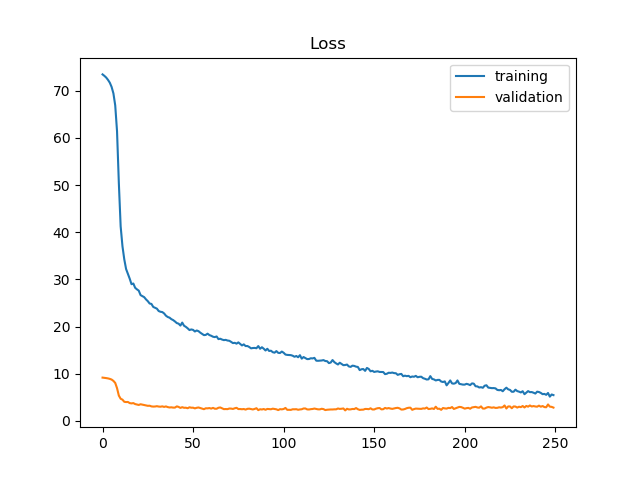
\includegraphics[width=0.5\textwidth]{Loss}
	\caption{Loss convergence}
	\label{fig:loss}
\end{figure}

\begin{figure}[h]
	\centering
	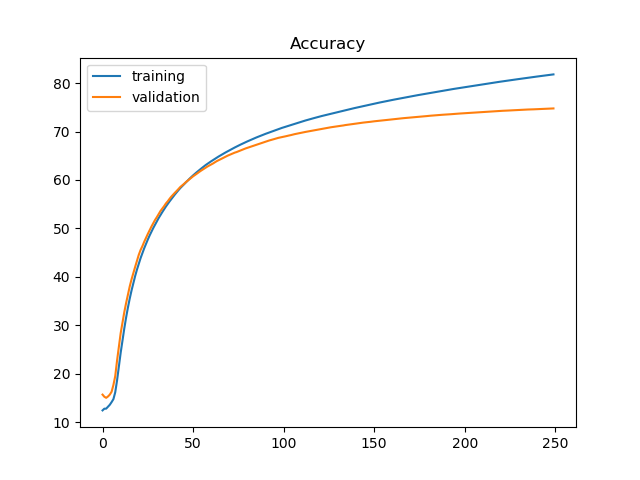
\includegraphics[width=0.5\textwidth]{Accuracy}
	\caption{Accuracy increase}
	\label{fig:accuracy}
\end{figure}

\section{Conclusion and future work}

In our work, we present a simple CNN architecture which is evaluated on CIFAR-Fruits datasets containing 4500 images. During the experiments, we have evaluated different architectures, and then choose one of them to tune further. Tuning the features of the parameters show good enhancement in performance. However, there may be certain improvements in the dataset. For instance, it took the whole one day to load the data which was not well represented because of merging two datasets. In addition, the number of images in the dataset could be increased either by adding more images from original datasets itself or by data augmentation which was not implemented at this time. Also, if we had more time we could try better architecture search using transfer learning with pretrained networks. Moreover, we will try weight decay in optimization technique and may consider better architecture search with certain hyperparameter initialization techniques like evolutionary strategies.

\bibliographystyle{IEEEtran}
\bibliography{reference}
\printbibliography

\end{document}